\documentclass[12pt,unicode]{beamer}
\usetheme{sakura}
\usepackage{luatexja-ruby}
\ltjsetparameter{%
    jacharrange={%
        -2, % Exclude Greek and Cyrillic letters.
        -3  % Punctuations and Miscellaneous symbols.
    },
    alxspmode={`/,allow},
    alxspmode={`#,allow},
    alxspmode={92,allow}
}
\usepackage{fontawesome}
\usepackage[sort]{natbib}
\defcitealias{poetics}{アリストテレス『詩学』1457b}
\defcitealias{ginga}{宮澤賢治『銀河鉄道の夜』九 ジョバンニの切符}
\usepackage{appendixnumberbeamer}
\usepackage{ccicons}
\usepackage{framed}
\usepackage[hang,flushmargin]{footmisc}
\usepackage{listings}
%https://tex.stackexchange.com/questions/24136/natbib-and-hyperref-for-author-year-style-produces-two-links/27235
\usepackage{etoolbox}
\usepackage{appendixnumberbeamer}

\makeatletter

\pretocmd{\NAT@citex}{%
  \let\NAT@hyper@\NAT@hyper@citex
  \def\NAT@postnote{#2}%
  \setcounter{NAT@total@cites}{0}%
  \setcounter{NAT@count@cites}{0}%
  \forcsvlist{\stepcounter{NAT@total@cites}\@gobble}{#3}}{}{}
\newcounter{NAT@total@cites}
\newcounter{NAT@count@cites}
\def\NAT@postnote{}

% include postnote and \citet closing bracket in hyperlink
\def\NAT@hyper@citex#1{%
  \stepcounter{NAT@count@cites}%
  \hyper@natlinkstart{\@citeb\@extra@b@citeb}#1%
  \ifnumequal{\value{NAT@count@cites}}{\value{NAT@total@cites}}
    {\ifNAT@swa\else\if*\NAT@postnote*\else%
     \NAT@cmt\NAT@postnote\global\def\NAT@postnote{}\fi\fi}{}%
  \ifNAT@swa\else\if\relax\NAT@date\relax
  \else\NAT@@close\global\let\NAT@nm\@empty\fi\fi% avoid compact citations
  \hyper@natlinkend}
\renewcommand\hyper@natlinkbreak[2]{#1}

% avoid extraneous postnotes, closing brackets
\patchcmd{\NAT@citex}
  {\ifNAT@swa\else\if*#2*\else\NAT@cmt#2\fi
   \if\relax\NAT@date\relax\else\NAT@@close\fi\fi}{}{}{}
\patchcmd{\NAT@citex}
  {\if\relax\NAT@date\relax\NAT@def@citea\else\NAT@def@citea@close\fi}
  {\if\relax\NAT@date\relax\NAT@def@citea\else\NAT@def@citea@space\fi}{}{}

\makeatother
\newenvironment{quoteblock}{%
    \def\FrameCommand{%
        {\color{sLightGray}{\vrule width 3pt}}%
        \hspace{10pt}
    }%
    \MakeFramed {\advance\hsize-\width \FrameRestore}}%
{\endMakeFramed}
\renewcommand\refname{参考文献}
\renewcommand\appendixname{付録}
\title{Lua\TeX{}-jaとbeamerで言語学関連のスライドを作る}
% \subtitle{副題}
\institute{総合研究大学院大学}
\author{宮澤 彬}
\date{{\number\year}年{\number\month}月{\number\day}日}
\hypersetup{%
    colorlinks,
    allcolors=sDarkBlue
}
\usepackage{gb4e,cgloss4e}
\noautomath%
\begin{document}

\begin{frame}[noframenumbering,plain]
    \maketitle
\end{frame}

\section{はじめに}
\begin{frame}
    \frametitle{はじめに}
    このスライドは \faGithub\ \href{https://github.com/pecorarista/sakuratheme}{\ttfamily pecorarista/sakuratheme}
    のデモとして作ったものです.

    \bigskip

    そのため作り方を詳しく説明することはしませんが,
    コードはすべて上記のレポジトリに含まれているので気になる方は参照ください.
    \bigskip

    また言語学関連の話題の\LaTeX における扱い方を網羅的に知りたい方は
    \href{https://www1.essex.ac.uk/linguistics/external/clmt/latex4ling/}
    {LaTeX for Linguists}が参考になります.
\end{frame}

\section{使用例}
\subsection{グロス}
\begin{frame}[fragile]
\frametitle{グロスI}
\href{https://ctan.org/pkg/gb4e}{\texttt{gb4e}}パッケージを利用します.

\bigskip

表示の不具合を防ぐため
    \texttt{cgloss4e.sty}を作業ディレクトリにコピーし\footnote[frame]{%
インストールされている場所がわからない場合はCTANからダウンロードしてください.
},以下のように変更します.
\begin{leftbar}
\begin{lstlisting}[%
    language={[LaTeX]TeX},
    basicstyle=\ttfamily\scriptsize,
    % asterisk for highlight backslash
    texcsstyle=*\color{sRed}\bfseries,
    keywordstyle=\bfseries,
    moretexcs={@ifundefined,eachwordone,eachwordtwo,eachwordthree},
    commentstyle=\color{sDarkBlue}
]
- \@ifundefined{eachwordone}{\let\eachwordone=\rm}{\relax}
+ \@ifundefined{eachwordone}{\let\eachwordone=\relax}{\relax}

- \@ifundefined{eachwortwo}{\let\eachwordtwo=\rm}{\relax}
+ \@ifundefined{eachwortwo}{\let\eachwordtwo=\itshape}{\relax}

- \@ifundefined{eachworthree}{\let\eachwordthree=\rm}{\relax}
+ \@ifundefined{eachworthree}{\let\eachwordthree=\relax}{\relax}
\end{lstlisting}
\end{leftbar}
\end{frame}

\begin{frame}[fragile]
\setlength{\glossglue}{5pt plus 2pt minus 1pt}\footnotesize
\frametitle{グロスII}
余白が狭く感じる場合は以下のように調整を行うとよいです.
\begin{leftbar}
\begin{lstlisting}[%
    language={[LaTeX]TeX},
    basicstyle=\ttfamily\footnotesize,
    % asterisk for highlight backslash
    texcsstyle=*\color{sRed}\bfseries,
    keywordstyle=\bfseries,
    moretexcs={setlength,glossglue},
    morekeywords={plus,minus},
    commentstyle=\color{sDarkBlue}
]
\setlength{\glossglue}{5pt plus 2pt minus 1pt}
\end{lstlisting}
\end{leftbar}

結果はこのようになります.
\begin{exe}
    \ex%
    \glll%
    {これは} {ロシア語の} {教科書} {です} \\
    {kore-wa} {rosia-go-no} {kyōkašo} {desu} \\
    {this-\textsc{top}} {Russia-language-\textsc{gen}} {textbook} {be} \\
    \trans%
    ``This is a textbook of the Russian language''
    \ex%
    \glll%
    {Это} {учебник} {русского} {языка} \\
    % {Э'то} {уче'бник} {ру'сского} {языка'} \\
    {èto} {učebnik} {russk-ovo} {jazyk-a} \\
    {this} {textbook.\textsc{sg.nom}} {Russian-\textsc{m.sg.gen}} {language-\textsc{gen}} \\
    \trans%
    ``This is a textbook of the Russian language.''
\end{exe}
\end{frame}


\begin{frame}[fragile]
\frametitle{ギリシャ文字やキリル文字を使うときの注意点}
Lua\TeX{}-jaパッケージを読み込んだときに注意しなければならないのが,
ギリシャ文字やキリル文字を和文フォントが表示されることです.
プリアンブルに以下を追加して欧文フォントで表示されるようにしましょう.
\begin{leftbar}
% https://tex.stackexchange.com/questions/17774/listings-package-can-i-include-a-backslash-in-language-keyword-begin-for
\begin{lstlisting}[%
    language={[LaTeX]TeX},
    basicstyle=\ttfamily\footnotesize,
    % asterisk for highlight backslash
    texcsstyle=*\color{sRed}\bfseries,
    keywordstyle=\bfseries,
    moretexcs={ltjsetparameter},
    morekeywords={jacharrange},
    commentstyle=\color{sDarkBlue}
]
\ltjsetparameter{%
  jacharrange={%
    -2,  % Exclude Greek and Cyrillic letters
    -3   % Exclude Punctuations and Misc symbols
  }
}
\end{lstlisting}
\end{leftbar}
\end{frame}

\subsection{音声記号}
\begin{frame}
    \frametitle{音声記号}
    Fira Sansフォントは多くの文字を含んでおり,またLua\LaTeX はユニコードによる入力に対応しているため,そのまま打ち込むだけで音声記号が表示されます.

    \smallskip

    (例)\textbf{медуза} [mʲɪˈduzə] くらげ

    \bigskip

    入力には以下を用いると便利です.
    \begin{itemize}
        \item Windows → \faGithub\ \href{https://github.com/samhocevar/wincompose}{\texttt{samhocevar/wincompose}}
        \item macOS → \faGithub\ \href{https://github.com/gnarf/osx-compose-key}{\texttt{gnarf/osx-compose-key}}
        \item Linux → 標準のCompose Key
    \end{itemize}
\end{frame}

\subsection{その他}
\begin{frame}
    \frametitle{画像の引用}
    画像の挿入には\texttt{\textbackslash includegraphics}コマンドを使います.
    Creative Commonsライセンスの作品には\texttt{ccicons}パッケージのアイコンを利用すると便利です.
    必要に応じて\texttt{\textbackslash href\{}\emph{uri}\texttt{\}\{}\emph{text}\texttt{\}}で元のファイルへリンクを張ります.

    \bigskip

    \begin{figure}[b]
        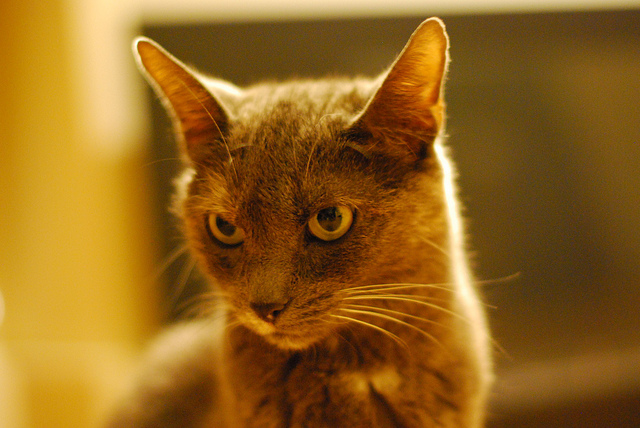
\includegraphics[width=0.4\textwidth]{cat.jpg}
        \caption{\href{https://www.flickr.com/photos/selda_eigler/8687127864/in/photolist-eeDNsC-qWFs4R-7CNDjJ-9c8DxY-eeDNhC-UCZ63T-dJNGUc-e5Nk39-988EVA-kUgwo-owDcVP-jQGjjt-5zkGTy-7WRCUo-b91XbZ-Mj8Ku-5pzwSA-9Bct2H-7CNHMY-7CJJMB-8MyEYn-9x45Mp-7JTq8M-ZrpGJ9-8fRht4-4SxVZT-5pzwjJ-ZsPJjL-aE44GL-dF6uWD-kqbHgM-5F373J-ZsQrVG-qyD7E9-ajyDPL-4WDvTp-KbDSc-5kCxD9-4MdeUo-pgDQcG-pPWrXD-662AFD-oTnC8k-apYceQ-nJSaaY-7CJLZv-7CJJMn-7CNFsU-XNMWkw-ccdtT9}{\emph{Cat} by Selda Eigler} \ccby.}
    \end{figure}

\end{frame}

\begin{frame}
    \frametitle{長め文章の引用}
    \href{https://ctan.org/pkg/framed}{\texttt{framed}}パッケージのleftbar環境を使うと引用であることが分かりやすくなります.

    \begin{quoteblock}
ἅπαν δὲ ὄνομά ἐστιν ἢ κύριον ἢ γλῶττα ἢ μεταφορὰ ἢ κόσμος ἢ πεποιημένον ἢ ἐπεκτεταμένον ἢ ὑφῃρημένον ἢ ἐξηλλαγμένον.

\hfill \citetalias{poetics}
    \end{quoteblock}

    \begin{quoteblock}
        「あの森\ruby{琴}{ライラ}の宿でせう。
        あたしきつとあの森の中には、
        むかしの大きなオーケストラの人たちが集まつていらつしやると思ふわ。
        まはりには青い孔雀やなんかたくさんゐると思ふわ。」
        女の子が答へました。

        \hfill \citetalias{ginga}
    \end{quoteblock}
\end{frame}

\begin{frame}[plain,noframenumbering,allowframebreaks]
\frametitle{参考文献}
\footnotesize
\bibliographystyle{jecon}
\bibliography{demo}
\end{frame}

\appendix
\begin{frame}
    \footnotesize
    \frametitle{\appendixname}
    箇条書きの項目が鉤括弧から始まるときの注意点
    \begin{itemize}
        \item こんてちあ
        \item 「こんてちあ」

            行頭の余白が大きい
        \item \leavevmode\inhibitglue 「こんてちあ」

            \texttt{\textbackslash item \textbackslash leavevmode\textbackslash inhibitglue} で余白を調整
    \end{itemize}

    \bigskip

    参照:\href{http://doratex.hatenablog.jp/entry/20140714/1405302796}{TeX Live 2014のpTeX系列における\textbackslash inhibitglueの仕様変更}
\end{frame}


\end{document}
